\documentclass{article}

\usepackage[inline]{enumitem}

\usepackage{url}
\usepackage{graphicx}
\graphicspath{ {./figures/} }

\title{Decentralised Mining Pool for Bitcoin}
\date{February 2021}

\begin{document}

\maketitle

\begin{abstract}
  Bitcoin p2pool's usage has steadily declined over the years and its
  decline impacts bitcoin's ability to remain decentralised. The
  primary problems with p2pool include large variance in earnings for
  miners, large number of dead on arrival blocks and the need for
  consuming valuable block space to reward miners.  BraidCoin and the
  use of channel payments are two proposals that have been put forward
  as possible means to alleviate these problems faced by p2pool. In
  this document, we present a unified solution that uses a directed
  acyclic graph to track miners shares and uses payments channels to
  reward miners. The shares calculation can be carried out by any of
  the p2p nodes, but the rewards are paid out by hubs. We show that
  our approach is incentives compatible and can reduce variance in
  earnings for miners. The approach presented here to use a DAG for
  tracking shares is a modified version of the proposal first put
  forward as BraidCoin.
\end{abstract}
   
\section{Motivation}

%% According to bitcoin wiki, 


%% \begin{quote}
%% P2Pool creates a new block chain in which the difficulty is adjusted
%% so a new block is found every 30 seconds. The blocks that get into the
%% P2Pool block chain (called the ``share chain'') are the same blocks
%% that would get into the Bitcoin block chain, only they have a lower
%% difficulty target. Whenever a peer announces a new share found (new
%% block in the P2Pool block chain), it is received by the other peers,
%% and the other peers verify that this block contains payouts for all
%% the previous miners who found a share (and announced it) that made it
%% into the P2Pool share chain. This continues until some peer finds a
%% block that has a difficulty that meets the Bitcoin network's
%% difficulty target. This peer announces this block to the Bitcoin
%% network and miners who have submitted shares for this block are paid
%% in the generation transaction, proportionally to how many shares they
%% have found in the last while.
%% \end{quote}

P2Pool~\cite{p2pool:wiki} helped decentralise bitcoin by enabling
miners to select which transactions they mined and thus avoid any
potential censorship by pool operators. However, the construction of
P2Pool faced a number of problems that slowly lead to miners
abandonding the pool.

\begin{enumerate}
  \item Large variance in earnings for miners.
  \item Large number of dead on arrival blocks.
  \item Large block space requirement.
\end{enumerate}

The first two problems are a direct consequence of the shares block
rate limited to 30 seconds. With one block possible every thirty
seconds, any increase in hashrate on P2Pool results in miners shares
competing to be the next block in the chain. There is a clear tension
in play here, increasing the block rate frequency doesn't scale the
throughput of the pool in terms of number of shares found, as most of
them are orphaned and the miners not being rewarded for those
orphans. Ethereum's inclusive protocols~\cite{inclusive-protocols}
help alleviate the problem for the Ethereum blockchain, where small
pools can work with a reduced variance in their
rewards as show in the analysis by McElrath~\cite{mcelrath:variance}.


\section{Current Proposals}

TerraHash Coin~\cite{mcelrath:variance}, Jute~\cite{jute} and
\cite{spectre} are some of the early attempts to use a DAG for faster
block times. However, these works focus on changing the consensus
layer of bitcoin itself, by allowing miners to produce shares that
have conflicting transactions and then applying rules to find a set of
transactions acceptable at various cuts of the DAG.\

We think it will be very hard to get such a proposal accepted by the
bitcoin community. Instead we focus on ``braiding the shares
chain''. That is we propose applying the principles of using a DAG to
enable faster block times to a shares chain, similar to P2Pool's share
chain.

\subsection{Hash Rate Futures}

TerraHash Coin~\cite{mcelrath:variance} introduced the idea of
generating a coin native to the shares chain and enabling miners to
hedge against the insecurities of bitcoin's hashrate and bitcoin's
price moving against them.

Smaller, more faster blocks, called beads help reduce the variance in
the earnings for miners. The key idea there is that if miners can
produce blocks faster, say within 1 to 2 second periods, and that
those blocks are accepted by the decentralised pool. Then the number
of their blocks that get orphaned reduces and therefore the variance
in their earnings are a function of the pool size goes reduces.

Miners in TerraHash Coin earn the coin native to the shares chain for
each share they find. These native coins are used as a commodity to
hedge against the uncertainties of the total network hashrate in the
future and/or the price of bitcoin. This idea has a small problem that
the instruments that help miners hedge their risks are designed and
honoured by centralised parties. [to confirm]: However, if we allow
miners to earn their reward from hubs for each bitcoin block the pool
mines \emph{and} hedge their TerraHash coins against uncertainty, then
maybe we can sell this to bitcoin miners.[/to confirm]

\subsection{Payment Channels For Rewards Payout}

Apart from the work for increasing block rates using DAGs,
Belcher~\cite{channels-for-rewards} proposes a different idea to help
decentralise mining deals with the problem of a paying miners from a
decentralised mining pool. P2Pool uses the coinbase tranasaction of a
block to pay out miners. Belcher shows how a scheme can be constructed
using payment channels between federated hubs to pay miners after a
block has been successfully mined. The payouts can be paid after a
long enough period, similar to the 100 blocks requirements for
spending from coinbase transactions. Miners can register with hubs
where bitcoin has been locked in to open payment channels to
miners. The construction presented by Belcher show how both miners and
hubs can't cheat and how the funders of the hub can earn a reward for
providing the services accounting, distributing rewards and keeping
the hub secure and attack resistant.

The ideas of the Hash Rate Futures and Payment Channels for Rewards
Payouts together present a potential path for rebooting P2Pool. In the
rest of the document we present a slightly modified version of
TerraHash Coin and show how the various components can work toegether.

\section{Decentralised Bitcoin Mining}

In this section we present a modified version of TerraHash Coin and
show how it can use payments channels with hubs to deliver a
decentralised mining pool for bitcoin.

\subsection{A DAG of Shares}

TerraHash Coin shows how smaller more frequent blocks can form a
directed acyclic graph (DAG) of blocks, with each block pointing to
one or more one previous blocks. In TerraHash Coin all blocks are
smaller bitcoin blocks, each with fewer transactions than a bitcoin
block. Blocks in TerraHash Coin can have transactions repeated in
different blocks. The TerraHash Coin proposal describes how repeated
and potentially some double spend transactions can be resolved to
decide on the state of the ledger at any cut of the DAG.\

The rewards that miners earn in TerraHash Coin is a coin native to
TerraHash Coin. This coin native to TerraHash Coin can then be swapped
for Bitcoin. The proposal suggest two alternatives to deliver this
swap. One approach is to burn the native coin and receive bitcoin. The
other approach is that the native coin can be swapped for bitcoin via
financial instruments like derivatives of the network's hash rate.

We propose taking a slightly different approach, where the blocks of a
DAG represent shares of the mining pool and are entire bitcoin blocks
as opposed to being smaller blocks.

\begin{figure}[h]
  \begin{center}
    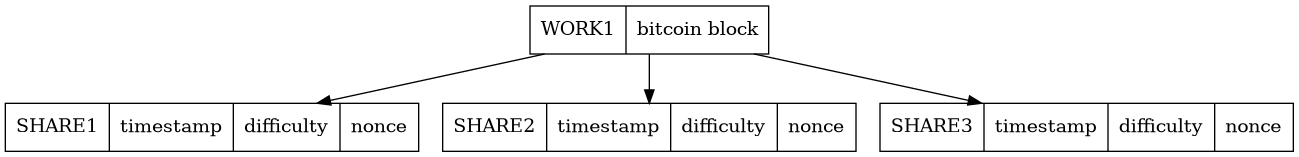
\includegraphics[width=1.0\textwidth]{work-share}
    \caption{Each \textsc{work} generated and shared by a miner is then
      followed by a number of \textsc{share}s the miner
      finds.}\label{fig:work-share}
    \end{center}
\end{figure}

Each miner builds their own block, selecting transactions as they
want, we call this ``\textsc{work}''. The description of \textsc{work}
is then disseminated to the p2p network of miners. The miner then
starts mining on \textsc{work} and generates ``\textsc{share}''. Each
\textsc{share} is mined at a difficulty level chosen by the
miner. This difficutly can be dynamically chosen by the miner after
each \textsc{share}, depending on what the miner observes on the p2p
network. This dynamic adjustment of difficulty is not included in our
proposal, but we note here that this is possible.

Figure~\ref{fig:work-share} shows the relationship between
\textsc{work} and its \textsc{share}s. Each \textsc{work} created by a
miner has multiple \textsc{share}s and they are both broadcast on the
p2p network.

The nodes in the DAG are \textsc{share}s mined at varied difficulty
levels. Each \textsc{share} that matches or exceeds the current
bitcoin difficulty starts a new $epoch$ for the p2p mining
pool. Figure~\ref{fig:epoch} shows $l$ and $r$ as the two valid
bitcoin blocks that have been mined such that they meet bitcoin's
difficulty at the time the block was mined, and all the blocks between
$l$ and $r$ are in the same $epoch$.

\begin{figure}[h]
  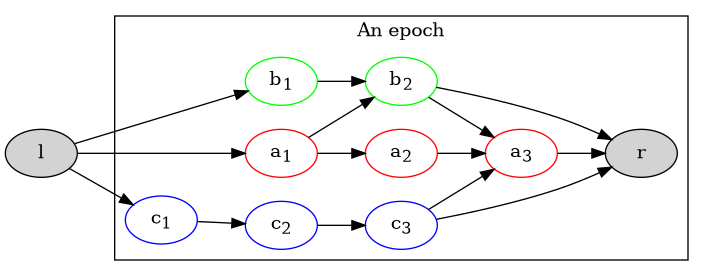
\includegraphics[width=1.0\textwidth]{epoch}
  \caption{A epoch is defined as all the \textsc{share}s mined between two
    bitcoin blocks. Here all the \textsc{share}s between $l$ and $r$ are in
    the same $epoch$.}\label{fig:epoch}
\end{figure}

\textsc{work} is created by miners and is shared with others on a peer
to peer network of miners using the compact
block~\cite{compact-blocks} specification. Each block created by a
miner is a valid bitcoin block, apart from the fact that it is mined
using a lower difficulty. The difficulty is chosen by the miner
creating the block such that it can mine blocks with their hash rate
to match the block rate of other miners in the p2p network.

When a miner starts working on a \textsc{share} it includes a
reference to the highest known \textsc{share} from all other miners
that the miner has receieved valid shares from. Note, the miner also
has access to \textsc{work} blocks from all participating miners. If a
miner doesn't have the \textsc{work} block from another miner, then it
rejects any \textsc{share}s received from the other miner. This is to
the deteriment of the other miners as we show in
Section~\ref{sec:rewards}.

In the next section we then describe how all peers compute their fair
share of profits using the DAG of shares. We show how our reward
computation algorithm is incentives
compatible~\cite{incentives-compatible}.

%% - block datastructure
%%   - coinbase reward goes to Hub's address
%%   - ignore this for now, we'll show how the reward is distributed in a
%%     trustless manner to all miners.
%% - DAG of shares
%%   - Epochs: start from and end with bitcoin block
%%   - Epoch ends when a valid bitcoin block with current bitcoin
%%     difficulty is found
%%   - Immediately send mined bitcoin block to bitcoin network
%%   - Hub will distribute the reward in around 100 blocks time
%% - Use compact blocks to inform others about the block we are mining
%%   - Other miners can decide to include your block as a previous block
%%     or not, whenever we find a solution and announce it.
%%   - We need to model the network traffic and latency
%% - Keep mining the same block, until end of epoch
%%   - For each block mined, share the solution with p2p network
%%   - Only if the mined block meets the current bitcoin difficulty
  
  
\subsection{Incentives Compatible Rewards}\label{sec:rewards}

Each participating node, which includes the miners and the hub, is
able to the see the DAG of \textsc{share}s as broadcast on the
network. Each \textsc{share} includes a reference to the blocks the
miner was aware of when the \textsc{share} was found. The reason for
doing so is simple. If a miner $a$ doesn't include the \textsc{share}s
of miner $b$, then $b$ has a clear signal to stop including the
\textsc{share}s of $a$, and as we will see a miner wants that their
\textsc{share}s are referenced by other miners as only then they will
be rewarded for their work.

The incentive in lay terms is that all miners should honestly include
the \textsc{share}s discovered by other miners, as otherwise they will
most likely be excluded by other miners and they will lose the
opportunity to be rewarded for their work. We call this the
degenerative case of ``isolated miners'' and argue that miners have no
incentives to act in this manner. Figure~\ref{fig:isolated-miners}
shows a DAG where all three miners $a$, $b$ and $c$ are working
independently. In such a situation when the miner $a$ discovers a
share and the reward is not shared with any other miner.

\begin{figure}[h]
  \begin{center}
    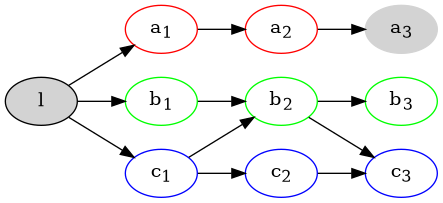
\includegraphics[width=0.5\textwidth]{isolated-miners}
    \caption{$a$ discovers a share and the reward is not shared with any
      other miner.}\label{fig:isolated-miners}
  \end{center}    
\end{figure}

With the above understanding of why miners will co-operate, we now
state the rules to calculate how the block reward should be divided
between miners.

\begin{enumerate}
  \item Traverse the DAG in reverse order from the \textsc{share} that
    found the latest bitcoin block to the previous bitcoin block found
    and collect a set of shares.
  \item From the above set of shares remove all shares that don't have
    a reverse path to the previous bitcoin block.
  \item Distribute the reward between miners weighted by the sum of
    the diffcultly of all \textsc{share}s found by miners.
\end{enumerate}

As an example consider the p2p network of miners $a$, $b$ and $c$ with
the DAG of shares as shown in Figure~\ref{fig:shares-dag}. In the DAG
the set of shares that receive reward proporitional to their
difficulty are $\{a_i..a_5, b_1..b_3\}$. The shares $\{c_1..c_3\}$ do
not receive any reward as they are not reachable from the bitcoin
block, $a_5$, even if they are reachable from $l$.

For the second bitcoin block $b_5$ only the miners $a$ and $b$ receive
rewards in proportion to the difficulties of their shares $\{b_4, b_5,
a_6\}$. $c$ doesn't receieve any reward for $c4$ as it is doesn't
include a reference to the last found bitcoin block $a_5$.

\begin{figure}[h]
  \begin{center}
    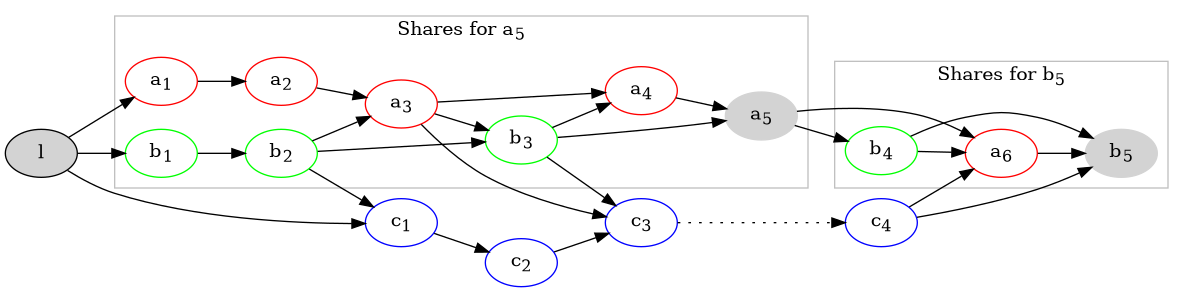
\includegraphics[width=1.0\textwidth]{shares-dag}
    \caption{Two epochs in a DAG of shares mined by three mines ---
      $a$, $b$ and $c$. The shares in grey meet the bitcoin difficulty
      at the time they were mined.}\label{fig:shares-dag}
  \end{center}
\end{figure}

With the above rules, it should be easy to prove that the rule reward
is an incentives compatible reward function as defined by
[ref:incentives compatibility], and we present an outline of proofs
that will be be formalised in future work.

\begin{description}
  \item [Incentive Compatibility] Given the rules above, if a miner
    finds a bitcoin block the miner wants to get maximum reward
    possible based on all the shares it has found and therefore is
    incentivized to announce their \textsc{share} as soon as they find
    it.
  \item [Proportional Payments] Since rewards are calculated at the
    end of an epoch, that is when all the valid shares found by all
    miners have been discovered, all miners are guaranteed payments
    for the shares that have reached the miner who found the block.
  \item [Budget Balanced] Again, since rewards are paid at the end of
    the epoch, a hub pays out rewards without losing or retaining any
    amount.
\end{description}

%% - Rewards computation
%%   - Rewards distribution
%%   - Incentives Compatible

\subsection{Payment Channels and Hubs}

The Hubs and payments channels proposal is exactly the same as that
described by Belcher~\cite{channels-for-rewards}. The only difference
is that Hubs calculate and distribute the rewards according to the
incentives compatible rewards scheme described above. We also adopt
the proposal that rewards are paid out after a 100 blocks of a block
being mined.

We would like to extend the proposal to include funding of hubs by
more than one party in a trustless manner, so that parties with small
BTC parties can engage in the peer to peer mining economy. This will
encourage faster adoption of our p2p mining network and make the
network stronger against DDoS attacks with multiple hub operators
available online.


%% \subsection{Implementation Plan}

%% The key components to build include:

%% 1. P2P shares network.
%%    1. Peers exchange both WORK blocks and SHARE
%%    blocks. The network is permissionless, i.e. anyone can join and
%%    start sharing their WORK and SHARE blocks.
%% 2. Rewards Computation.
%%    1. An algorithm to compute rewards.
%% 3. Hub.
%%    1. Create channels with p2p miners.
%%    2. Compute reward and distribute them.
%%    3. Connect to other hubs using a p2p or a rqelay network.
   

\section{Future Work}

\subsection{Proofs}

We want to use the model presented by Boneh et.al.\ to provide proofs
for how the rewards distribution is incentives compatible.

\subsection{Simulations}
Before we work on implementing they system, our next step is to
simulate p2p mining network using ns-3 [ref] and make informed
decisions about how large a network each hub will want to support. The
observations we want to make are how large a p2p network can be
sustained without an increase in work lost by miners. Each hub and p2p
network can grow as long as miners are communicate WORK and SHARES
with each other with bounded latency and can limit their lost
work. With a simulation we want to find out the bounds of these.

\subsection{Specifications and Implementation}

We want to specify the p2p protocol messages and the rules more
precisely. We also plan to implement the specifications and we expect
the two tasks to proceed hand in hand.

\bibliography{proposal} 
\bibliographystyle{acm}

\end{document}
